\documentclass{article}
\usepackage[framed,numbered,autolinebreaks,useliterate]{mcode}
\usepackage[utf8]{inputenc}
\usepackage[T1]{fontenc}
\usepackage[polish]{babel}
\usepackage{lmodern}
\selectlanguage{polish}
\usepackage{float}
\usepackage{hyperref}
\usepackage{color}
\usepackage{graphicx} 
\usepackage{float}
\hypersetup{
    colorlinks,
    citecolor=black,
    filecolor=black,
    linkcolor=black,
    urlcolor=black
}
\author{Bartosz Rajkowski}
\title{Projekt I STP\\zadanie 1.9}
\date{30 kwietnia 2017}

\begin{document}
\maketitle
\newpage
\tableofcontents
\newpage

\section*{Dane}
$$
G(s)=\frac{0,5s^2+3,5s+5,625}{s^3+8s^2-36s-288}
$$
\section{Zadanie 1}
\subsection{Treść}

Wyznaczyć transmitancję dyskretną $G(z)$, stosując ekstrapolator zerowego rzędu i przyjmując okres próbkowania $T_p=0,1s$. Określić zera i bieguny obydwu transmitancji. Odpowiedzieć na pytanie, czy obiekt jest stabilny.

\subsection{Program}
\lstinputlisting[caption={zad1.m}, label={lst:zad1}]{../zad1.m}
\subsection{Wyniki}
\subsubsection{Transmitancja dyskretna}
$$
G(z)=\frac{0.05183 z^2 - 0.07375 z + 0.0259}{z^3 - 2.82 z^2 + 2.065 z - 0.4493}
$$
\subsubsection[Bieguny i zera]{Bieguny i zera transmitancji ciągłej i dyskretnej}
\begin{enumerate}
\item Transmitancja ciągła
\begin{itemize}
\item Bieguny: \verb+6 -8 -6+
\item Zera: \verb+-4.5 -2.5+
\end{itemize}

\item Transmitancja dyskretna
\begin{itemize}
\item Bieguny: \verb+1.8221 0.5488 0.4493+
\item Zera: \verb+ -4.5 -2.5+
\end{itemize}
\end{enumerate}

\begin{figure}[t]
\centering
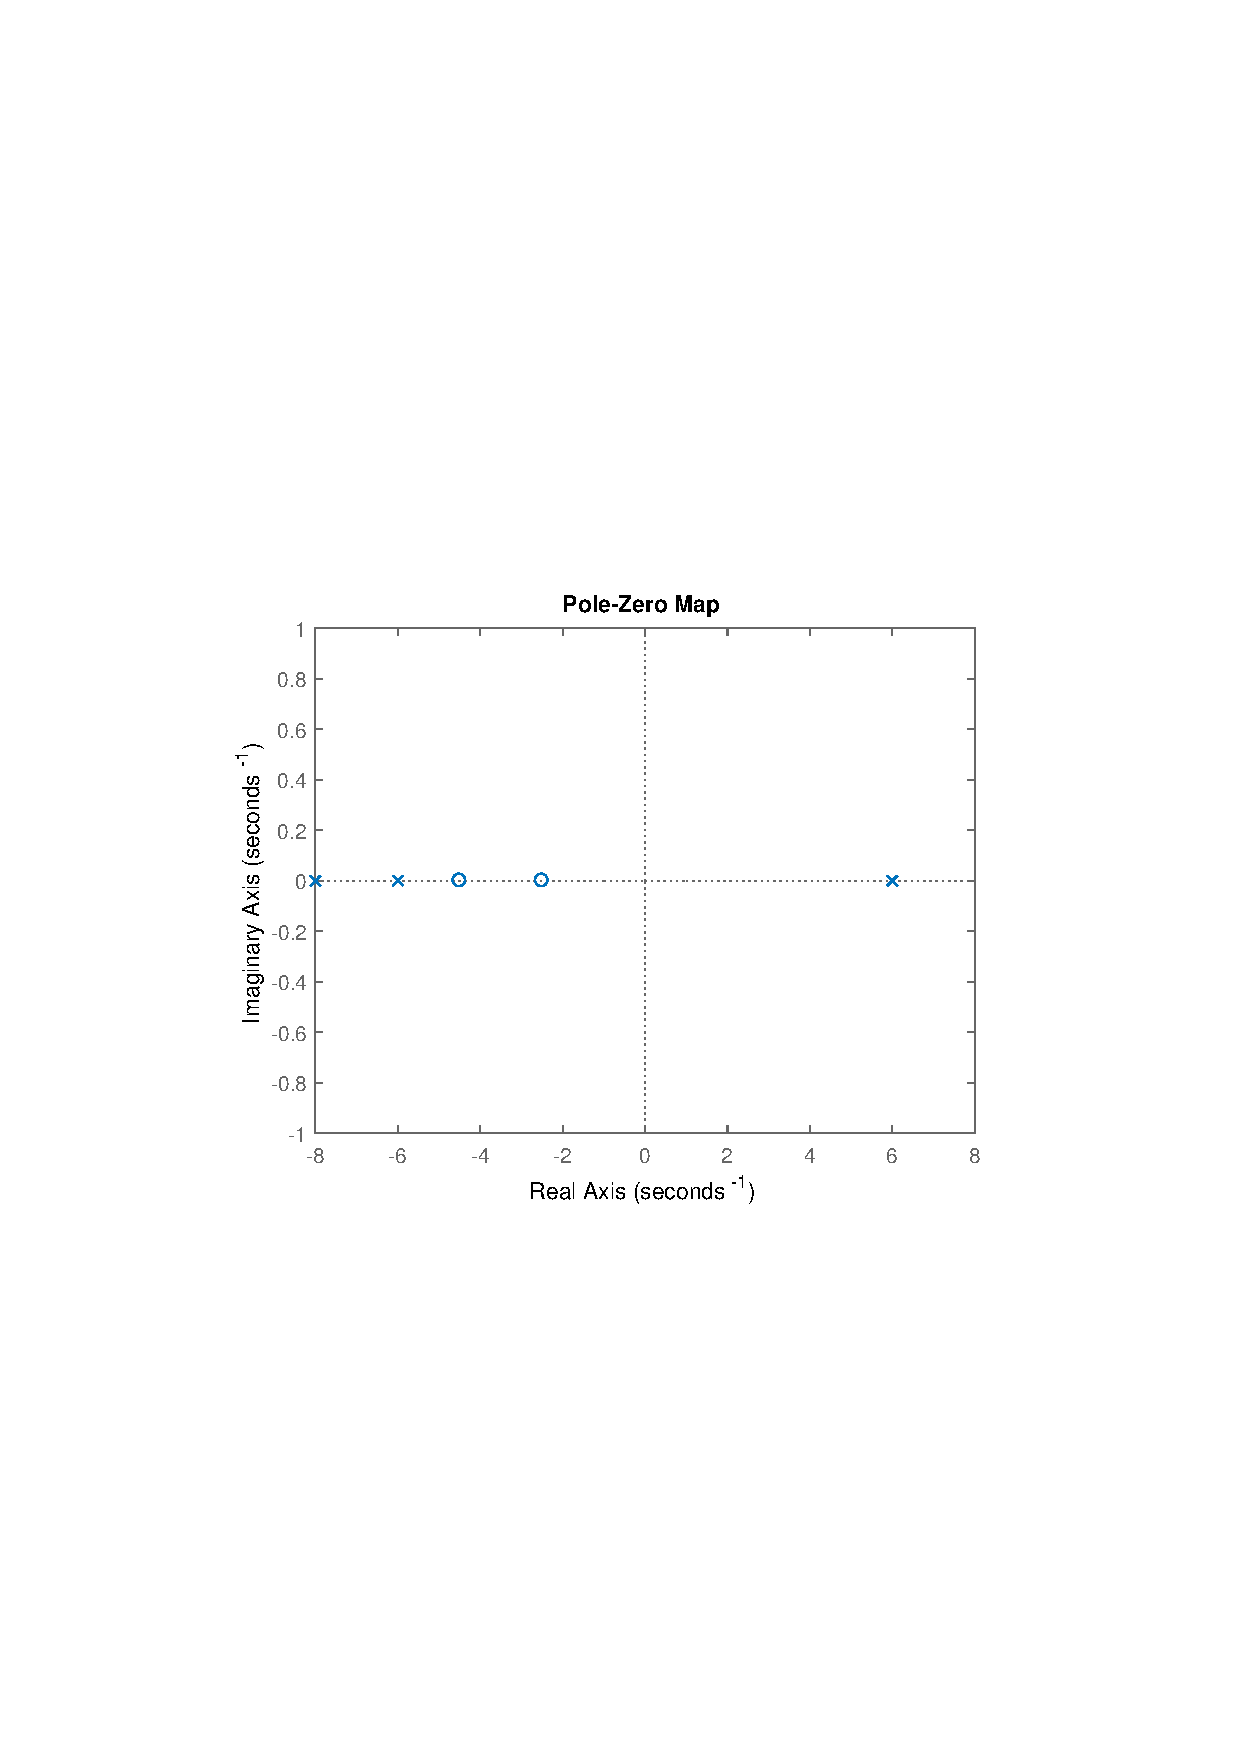
\includegraphics[width=10cm]{../rys/rys1}
\caption{Zera i bieguny transmitancji ciągłej}
\label{fig:rys 1}
\end{figure}

\begin{figure}[H]
\centering
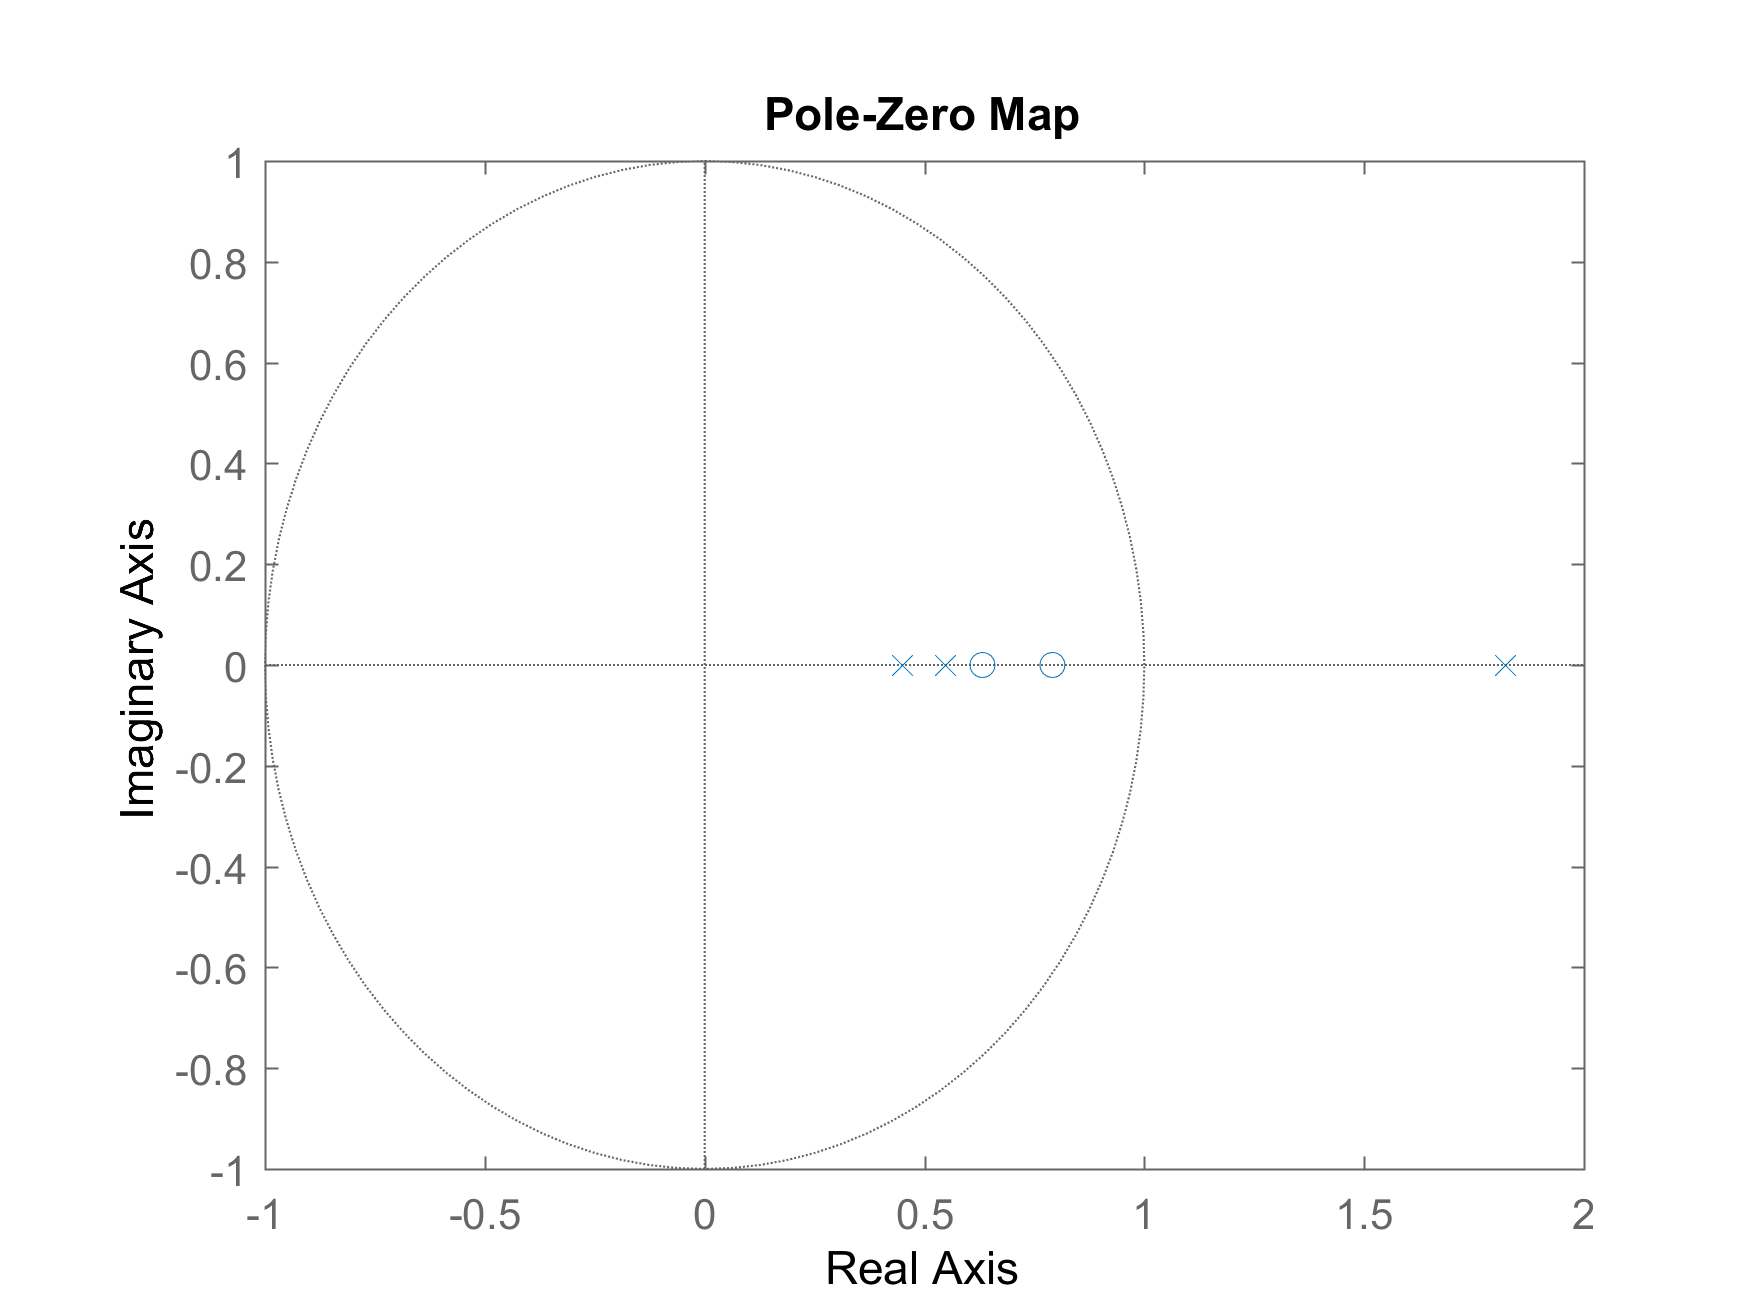
\includegraphics[width=10cm]{../rys/rys2}
\caption{Zera i bieguny transmitancji dyskretnej}
\label{fig:rys 2}
\end{figure}

\subsubsection{Wnioski}
Układ dyskretny jest stabilny tylko wtedy, gdy wszystkie jego bieguny leżą w~kole o promieniu 1 i środku w początku układu współrzędnych. Jak widać na~rysunku jeden z biegunów leży poza kołem, zatem układ nie jest stabilny.
\subsection{Zadanie 2}
\subsubsection{Treść}
Znaleźć reprezentację modelu dyskretnego w przestrzeni stanów stosując dwa warianty
metody bezpośredniej wyznaczania równań stanu na podstawie transmitancji, a następnie
narysować schematy otrzymanych modeli.
\subsection{Sposób rozwiązania}
Transmitancję dyskretną można obliczyć ze wzoru:
$$
G(z)=C(zI-A)^{-1}B+D
$$
W Matlabie służy do tego polecenie \verb+tf2ss+.
Wariant drugi od pierwszego różni się tym, że w rezultacie otrzymujemy macierze transponowane.
\subsection{Program}
\lstinputlisting[caption={zad2.m}, label={lst:zad2}]{../zad2.m}
\subsection{Wyniki}
\vbox{\begin{itemize}
\item wariant pierwszy\\\\
\begin{tabular}{l}
$
A=\left[\begin{array}{ccc} 2.82 & -2.065 & 0.4493\\ 1 & 0 & 0\\ 0 & 1 & 0 \end{array}\right]
$\\\\
$
B=\left[\begin{array}{c} 1\\ 0\\ 0 \end{array}\right],
C=\left[\begin{array}{ccc} 0.05183 & -0.07375 & 0.0259 \end{array}\right],
D=0
$
\end{tabular}
\item wariant drugi\\\\
\begin{tabular}{l}
$
A=\left[\begin{array}{ccc} 2.82 & 1 & 0\\ -2.065 & 0 & 1\\ 0.4493 & 0 & 0 \end{array}\right]
$\\\\
$
B=\left[\begin{array}{ccc} 1 & 0 & 0 \end{array}\right],
C=\left[\begin{array}{c} 0.05183\\ -0.07375\\ 0.0259 \end{array}\right],
D=0
$
\end{tabular}
\end{itemize}}

\end{document}